\input ../SlidePreamble
\input ../preamble

\begin{document}

{\Huge
  \centerline{\bf TTIC 31230,  Fundamentals of Deep Learning}
  \vfill
  \centerline{David McAllester, Autumn 2023}
  \vfill
  \centerline{\bf A Timeline of Deep Learning}
  \vfill
  \centerline{\bf and A Course Overview}
\vfill
\vfill


\slide{Early History}

{\bf 1943}: McCullock and Pitts introduced the {\color{red} linear threshold ``neuron''}. Words in red are important --- we will discuss them in detail in this class.

\vfill
{\bf 1962}: Rosenblatt applies a ``Hebbian'' learning rule.  Novikoff proved the perceptron convergence theorem.

\vfill
{\bf 1969}: Minsky and Papert publish the book {\it Perceptrons}.

\vfill
The Perceptrons book greatly discourages work in artificial neural networks.  Symbolic methods dominate AI research through the 1970s.

\slide{80s Renaissance}

{\bf 1980}: Fukushima introduces the neocognitron --- a form of {\color{red} convolutional neural Network or CNN}.  CNNs created the deep revolution in 2012.

\vfill
{\bf 1984}: Valiant defines PAC learnability and stimulates learning theory. Wins the Turing Award in 2010.

\vfill
{\bf 1985}: Hinton and Sejnowski introduce the Boltzman machine

\vfill
{\bf 1986}: Rummelhart, Hinton and Williams demonstrate empirical success with {\color{red} backpropagation} (itself dating back to 1961).

\slide{90s and 00s: Research In the Shadows}

{\bf 1997}: Schmidhuber et al. introduce LSTMs (a form of {\color{red} recurrent neural network or RNN}).

\vfill
{\bf 1998}: LeCunn draws attention to convolutional neural networks (CNNs) (LeNet).

\vfill
{\bf 2003}: Bengio introduces {\color{red} neural language modeling}.

\slide{Current Era: 2012-13}

{\bf 2012}: Alexnet dominates the Imagenet computer vision challenge.

\vfill
Google speech recognition converts to deep learning.

\vfill
Both developments come out of Hinton's group in Toronto.

\vfill
{\bf 2013}: Refinement of AlexNet continues to dramatically improve computer vision.

\slide{2014}

{\bf 2014}: Neural machine translation appears (Seq2Seq models).

\vfill
{\color{red} Variational auto-encoders} (VAEs) appear.

\vfill
{\color{red} Generative Adversarial Networks} (GANs) appear.

\vfill
{\color{red} Graph neural networks appear} (GNNs) revolutionizing the prediction of molecular properties.

\vfill
Dramatic improvement in computer vision and speech recognition continues.

\slide{2015-16}

{\bf 2015}: Google converts to neural machine translation leading to dramatic improvements.

\vfill
{\color{red} Batch Normalization} appears improving the performance of image classification.

\vfill
{{\color{red} Residual Connections} appear.  This makes yet another dramatic improvement in computer vision.

\vfill
{\color{red} Diffusion Models} are formulated which become important in 2021.

\vfill
{\bf 2016}: {\color{red} Reinforcement Learning} is used to develop Alphago which defeats Lee Sedol.

\slide{2017}

{\bf 2017}: AlphaZero learns both go and chess at super-human levels in a mater of hours entirely form self-play and advances computer go far beyond human abilities.

\vfill
Unsupervised machine translation is demonstrated.

\vfill
Progressive GANs demonstrate high resolution realistic face generation.

\vfill
The {\color{red} Transformer} appears greatly improving language modeling.

\slide{2018}

{\color{red} Unsupervised pre-training} significantly improves a broad range of NLP tasks including question answering.

\vfill

{\color{red} Contrastive learning} is formulated which ultimately becomes the foundation of various systems.

\vfill
AlphaFold revolutionizes protein structure prediction.

\slide{Progress on GANS}
\centerline{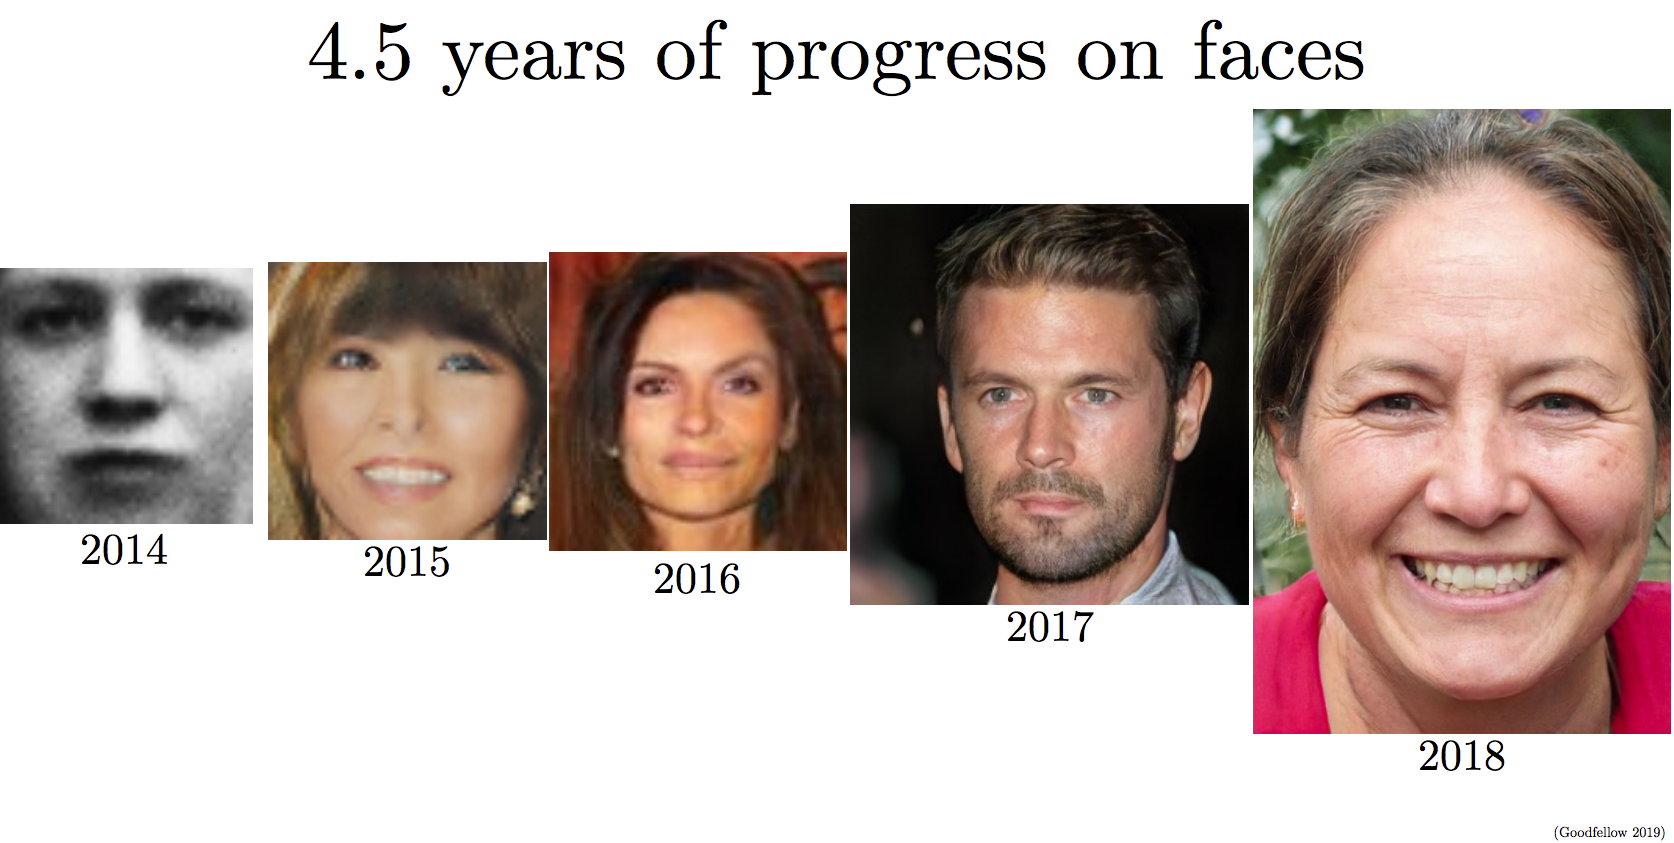
\includegraphics[height = 4.0in]{\images/GoodfellowInvited1}}

ArXiv 1406.2661, 1511.06434, 1607.07536, 1710.10196, 1812.04948

\centerline{Goodfellow, ICLR 2019 Invited Talk}

\slide{Progress on GANs}

\centerline{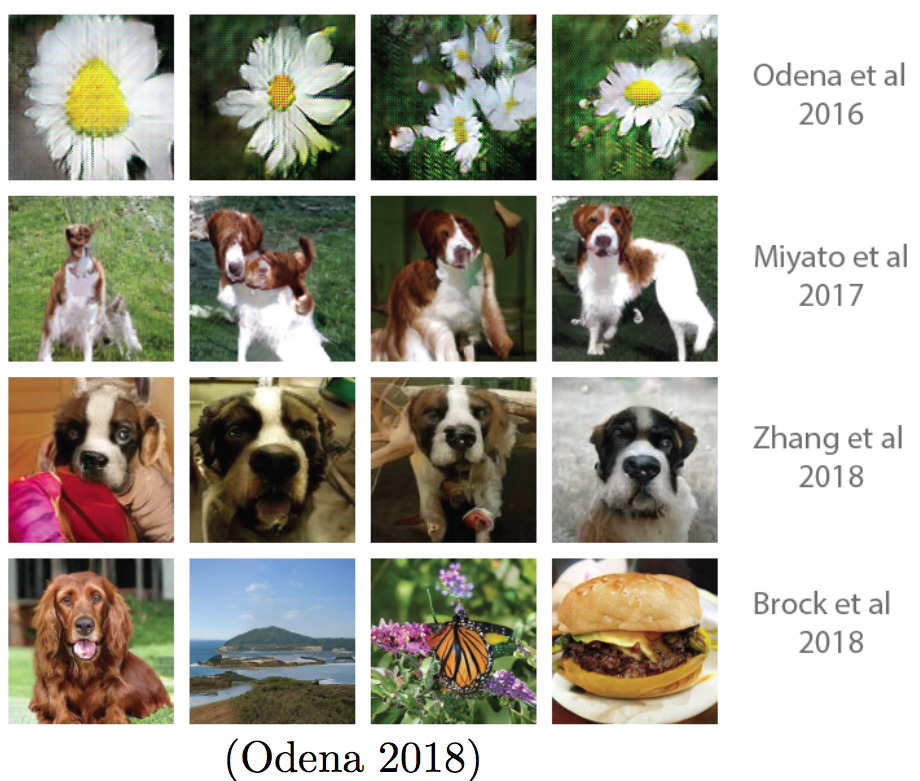
\includegraphics[height = 5.0in]{\images/GoodfellowInvited2}}

\slide{BigGANs, Brock et al., 2018}

\centerline{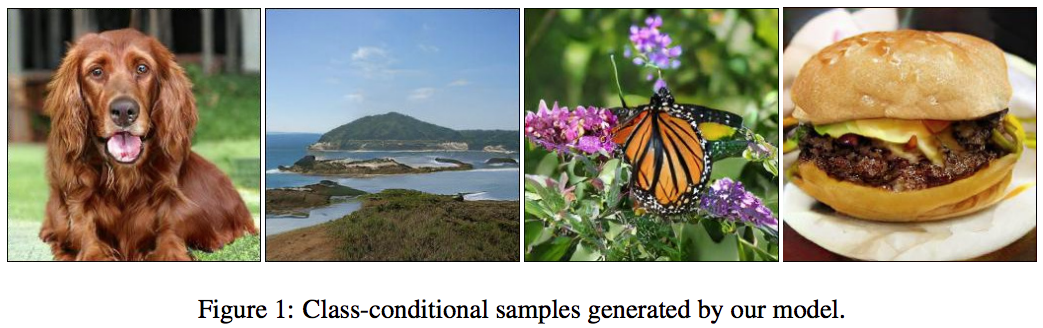
\includegraphics[width = 10.0in]{\images/BigGANs}}

\slide{Variational Auto Encoders (VAEs, 2015)}

\centerline{\includegraphics[width = 4in]{\images/VariationalFaces}}
\centerline{[Alec Radford, 2015]}

\slide{2019: Vector Quantized VAEs}

\centerline{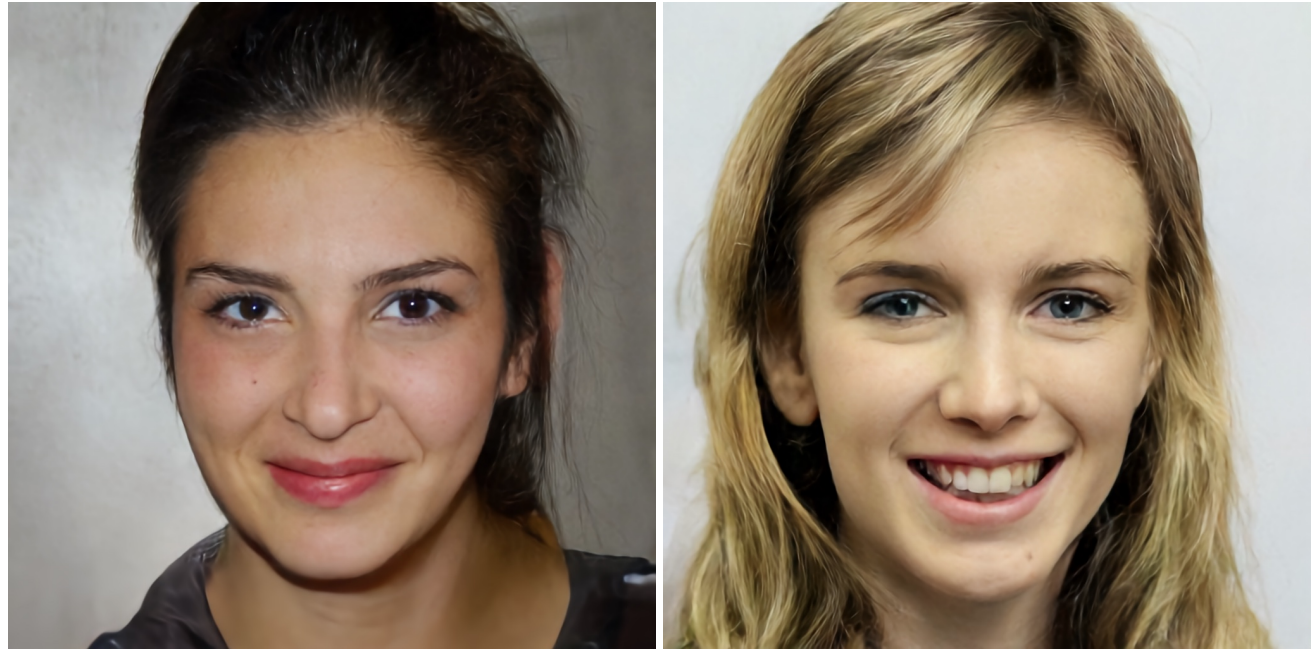
\includegraphics[width = 8in]{\images/VQ-VAE22}}

\vfill
VQ-VAE-2, Razavi et al. June, 2019

\slide{VAEs in 2019}

\centerline{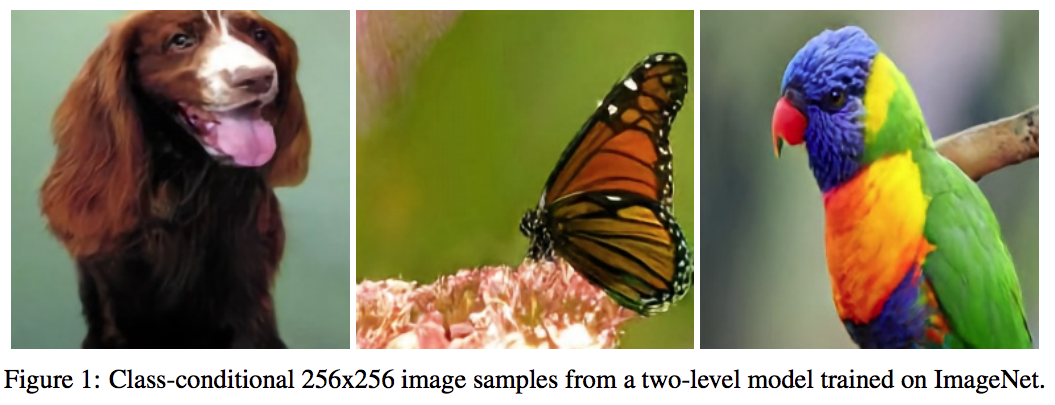
\includegraphics[width = 10in]{\images/VQ-VAE21}}

\vfill
VQ-VAE-2, Razavi et al. June, 2019

\slide{2019: Natural Language Understanding}

GLUE: General Language Understanding Evaluation

\centerline{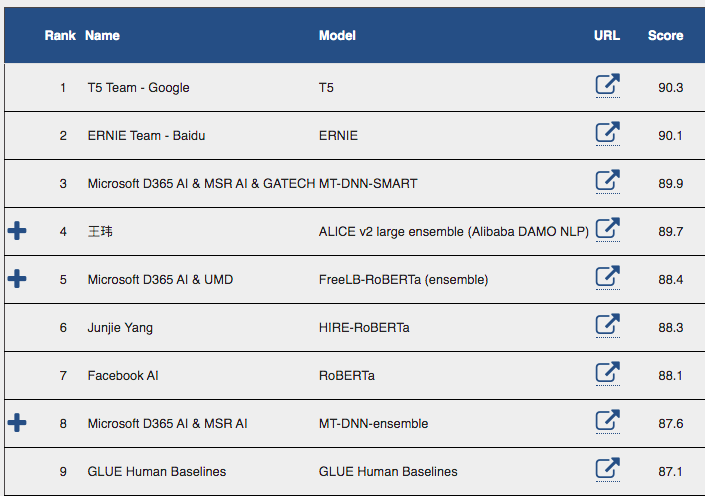
\includegraphics[width= 6in]{\images/GLUELeader}}

\slide{June 2020: Wav2vec 2.0, Facebook}

\vfill
Trained on 53k hours of unlabeled audio (no text) they use {\color{red} contrastive learning} to convert speech to a sequence of discrete {\color{red} quantized vectors} they call ``pseudo-text units''.

\vfill
By training on only one hour of human-transcribed audio, and using the Wav2vec transcription into pseudo-text, the outperform the previous state of the
art in word error rate for 100 hours of human-transcribed text.


\slide{February 2021: GLSM,  Facebook}

Generative Spoken Language Model (GSLM)

\vfill
Using a form of {\color{red} VQ-VAE} They then train a generative model of the sequences of pseudo-text units learned from unlabeled audio.


\vfill
This model can continue speech from a speech prompt in much the same way that GPT-3 continues text from a text prompt.

\vfill
Semantic and grammatical structure in a ``unit language model'' is recovered
from speech alone.


\slide{January 2021: CLIP, OpenAI}

CLIP: {\color{red} Contrastive} Language-Image Pre-training.

\vfill
Trained on images and associated text (such as image captions or hypertext links to images) CLIP computes embeddings of text and embeddings of images
(``co-embeddings'') trained to capture the mutual information between the two.

\vfill
This is done with contrastive learning.

\slide{CLIP}

The model computes a probability of text given the co-embedding of the image.

\vfill
It is then used for zero-shot image classification on various datasets.

\vfill
One can classify an image by comparing the probabilities that the model assigns to ``prompts''.  There is a prompt for each class.

\slide{Zero-Shot Image Classification}

\centerline{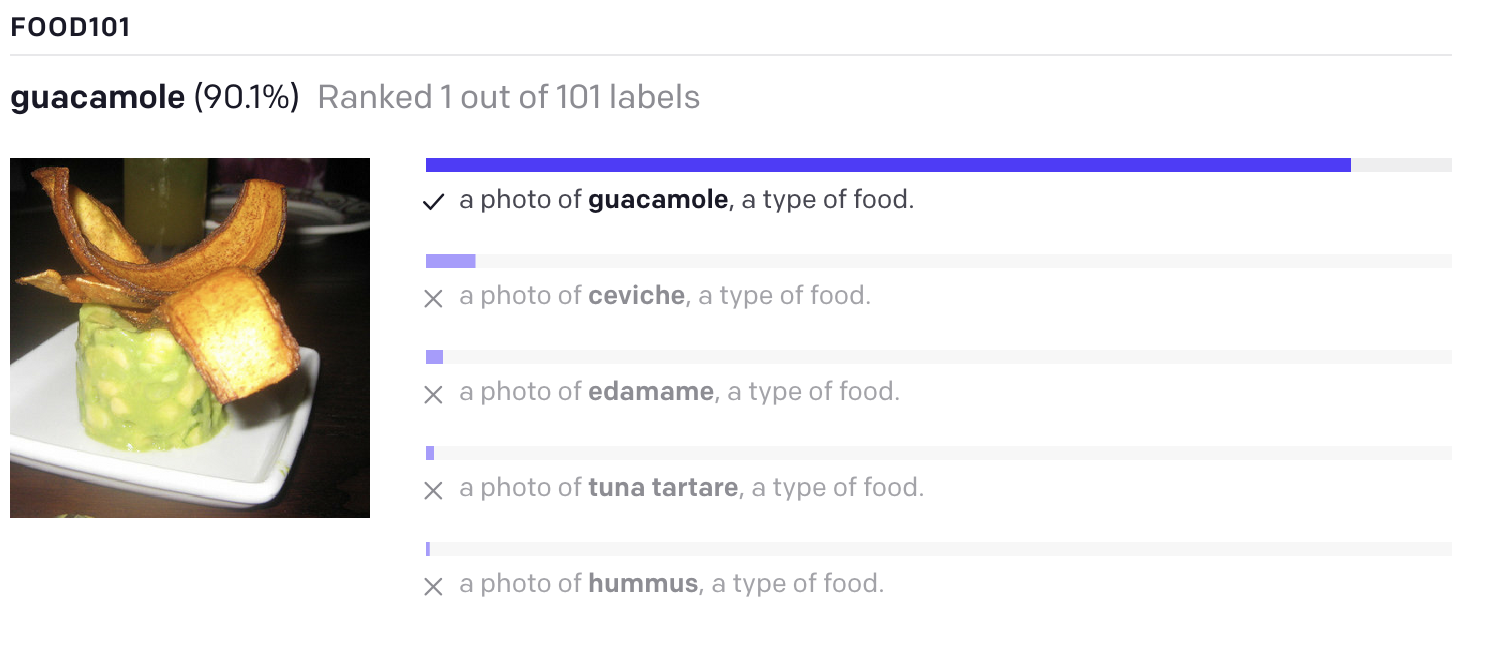
\includegraphics[width = 7in]{\images/CLIP0}}

\slide{Zero-Shot Image Classification}

\centerline{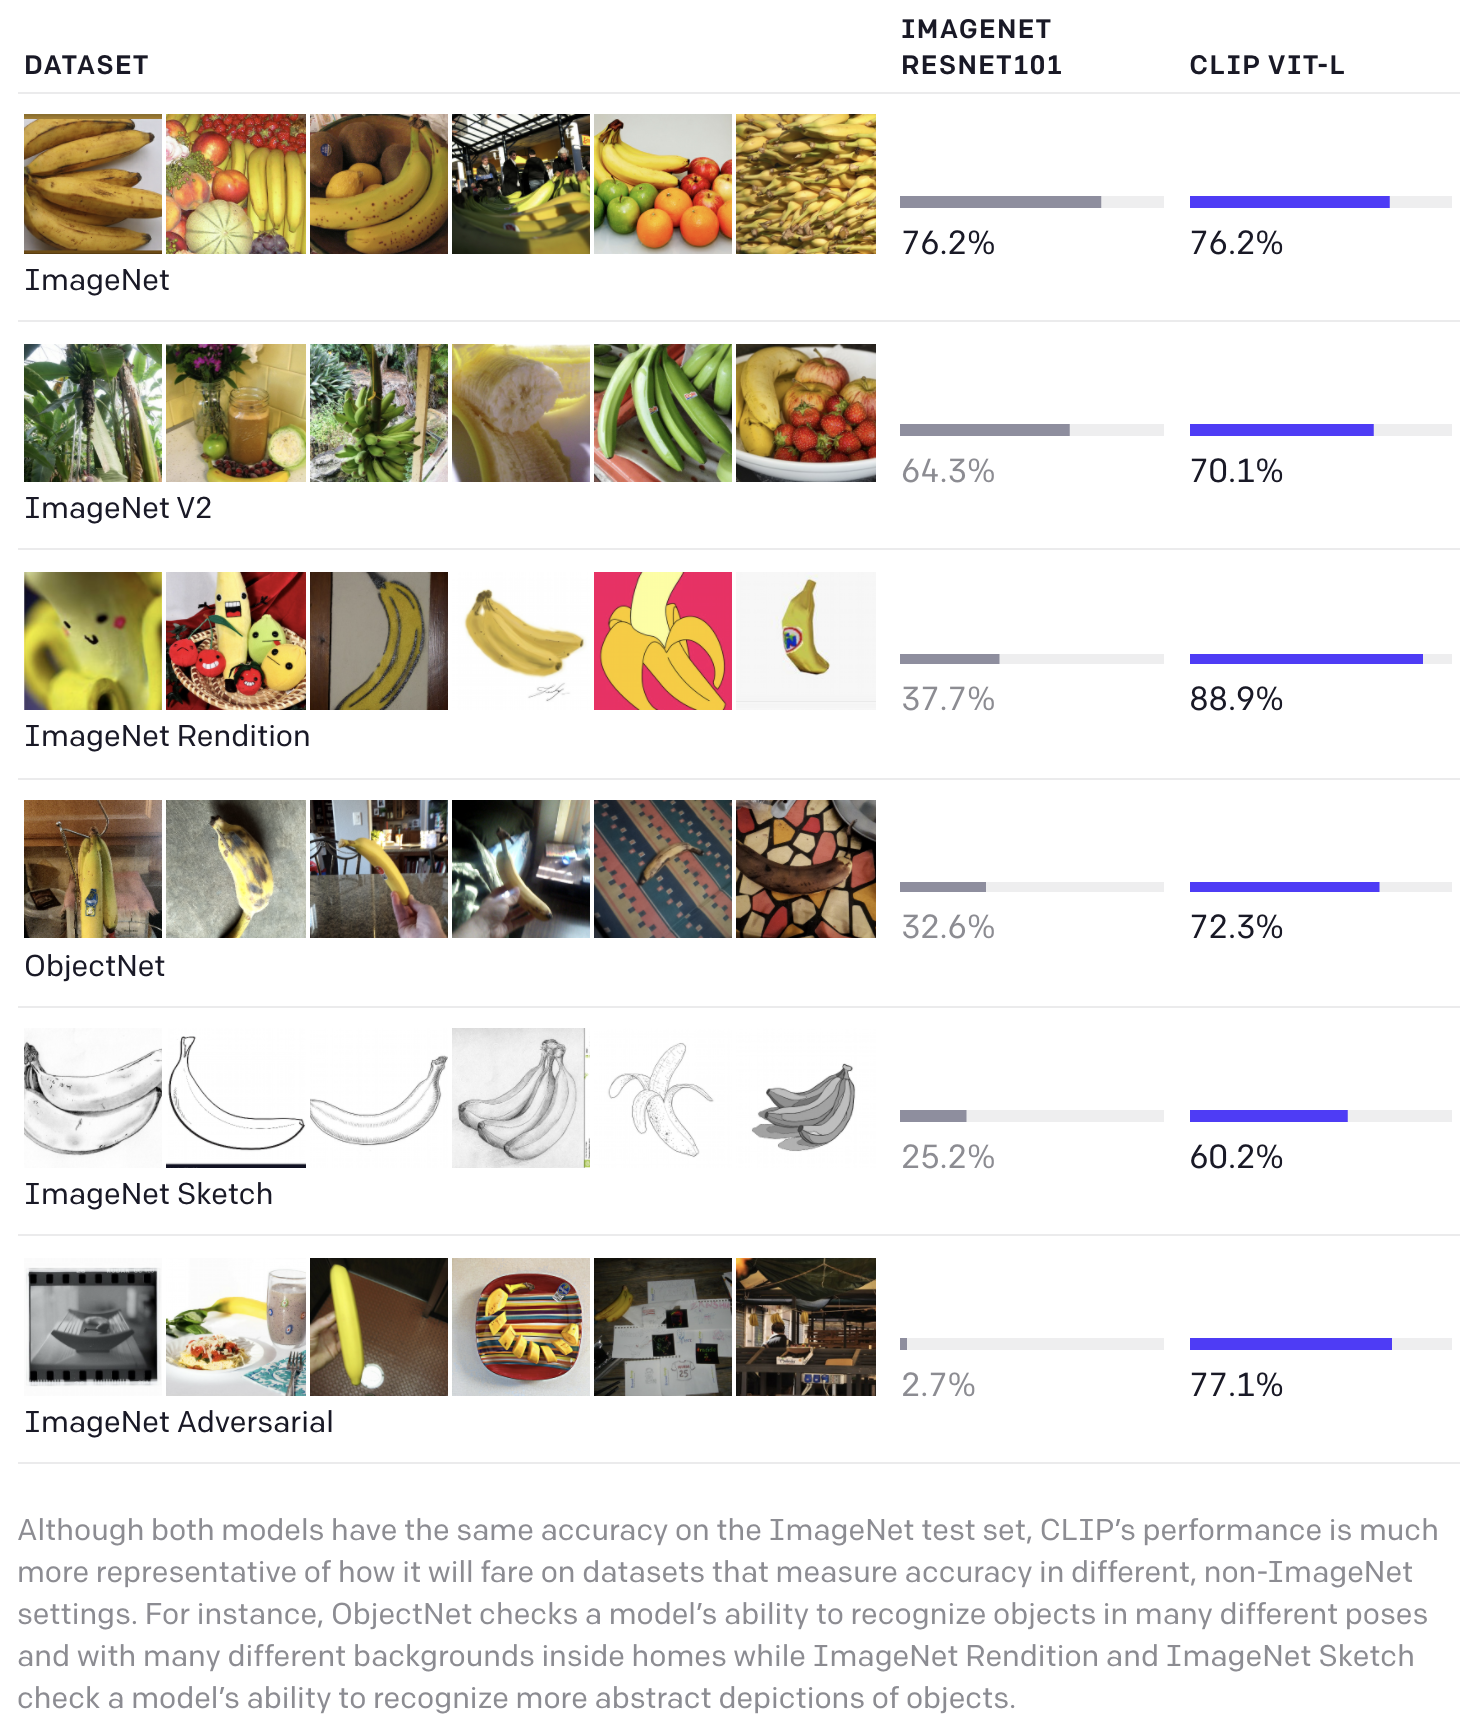
\includegraphics[height= 5in]{\images/CLIP1}}

\slidetwo{January 2021: DALL$\cdot$E, OpenAI}{April 2021: DALL$\cdot$E-2}

The name DALL$\cdot$E is simply some kind of homage to the painter Dali and the Disney character WALL$\cdot$E.

\vfill
Both versions of DALL$\cdot$E uses CLIP's co-embeddings of images and text.

\vfill
Given text, DALL$\cdot$E generates an image using a {\color{red} diffusion model}.

\slide{DALL$\cdot$E-1 Zero-Shot Image Rendering from Language}

\centerline{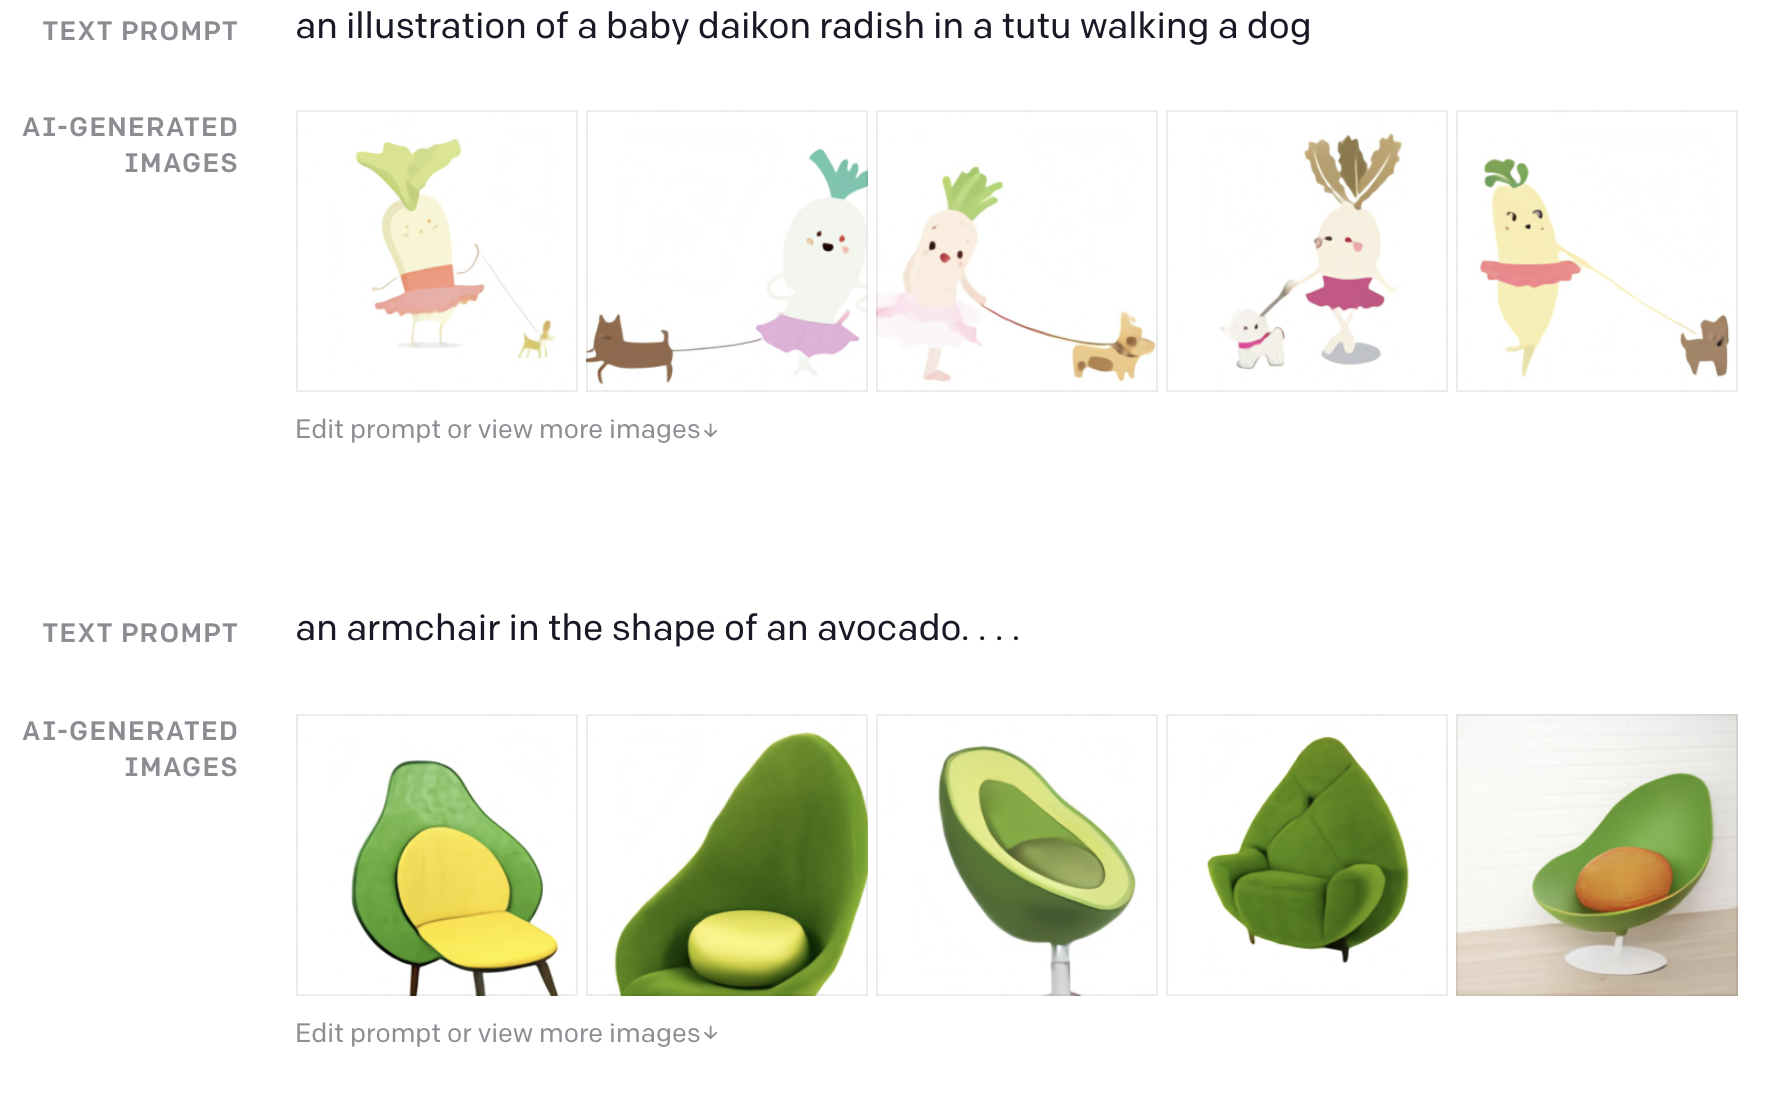
\includegraphics[height= 5in]{\images/DALLE1}}

\slide{DALL$\cdot$E-2}

\centerline{\includegraphics[height= 5in]{\images/DALLE2}}

\slide{July 2021: Codex, OpenAI}

Using an {\color{red} unsupersided pretrained language model} they fine-tune on code, including comments, from public repositories.

\vfill
Starting from an English prompt Codex continues with code --- a form of automatic programming.

\vfill
There is a published version (58 authors) and a production version that powers {\bf GitHub Copilot}.

\vfill
Copilot may supplant Stack Overflow for finding out how to do x in language y.

\slide{January 2022: Chain of Thought Prompting}

Give examples of {\color{red} ``chains of thought''} for few shot learning of reasoning steps.

\slide{Naive Prompting}

\centerline{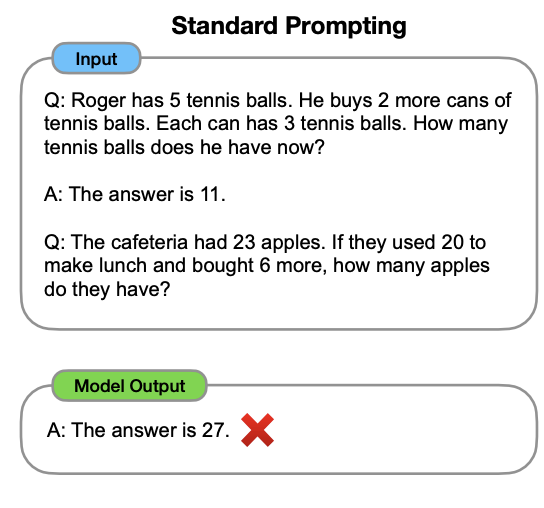
\includegraphics[height= 5in]{\images/ChainofThought1}}

\slide{Chain of Thought Prompting}

\centerline{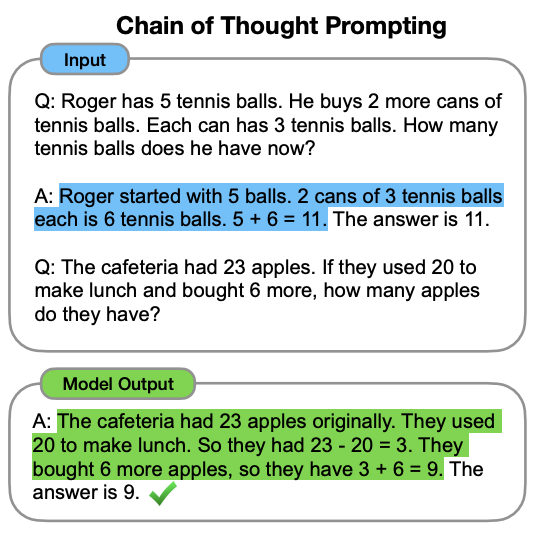
\includegraphics[height= 5in]{\images/ChainofThought2}}

\slide{June 2022: Step by Step Prompting}

It turns out that adding the simple instruction ``take it step by step'' elicits powerful chain of thought reasoning in GPT-3.

\slide{September 2022: Humanoid Soccer, Deep Mind}

Deep mind demonstrated two-on-two humanoid soccer in simulation (MuJoCo).

\vfill
This a startling advance in the state of the art in humanoid control.

\vfill
It also continues Deep Mind's effort in reinforcement learning.

\slide{March 2023: GPT-4 is Unveiled}

Dramatic improvement in conversational abilities and apparent understanding of common sense language meaning.

\vfill
Training involves ``instruction training'' and ``reinforcement learning with human feedback'' (RLHF).

\vfill
Most technical details are proprietary.

\vfill
GPT-4 shows both a tendency to ``hallucinate'', presenting fiction as fact,
and people find ways to ``jailbreak'' GPT4 into alternate and even malevolent personalities 

\vfill
Concerns over AI safety grows. Not everyone is concerned.

\slide{September 2023}

DALL$\cdot$E-3 has just been announced.

\vfill
ChatGPT continues to evolve. There is a new blog post from OpenAI today (Sept 26, 2023).

\vfill
Significant advances in speech recognition and speech generation continue.

\slide{Open Problems}

{\bf The MathZero Problem:} Since the development of AlphaZero people have been asking if the same thing could be done for the ``game'' of mathematics.

\vfill
{\bf The Autoformalization Problem:} This is the problem of automatically formalizing and verifying published proofs in mathematics possibly discovering legitimate gaps in the proofs where they exist.

\vfill
{\bf The Proof Assistant Problem:} This is the more modest goal of improving the level of automation in formal verification systems.  The system
most widely adopted by the mathematics community is LEAN based on dependent type theory.

\slide{Application Advancements vs. Architecture Advancements}

Advancements in the general principles of learning are having applications over very diverse applications.

\vfill
When considering Moore's law of AI it seems worth distinguishing architectural advancements (new general learning methods)
from new applications of established architectures or fine tuning of known methods.

\vfill
This course will focus on general, architectural, ideas.

\slide{Architectural Ideas}

\begin{itemize}
\item {\color{red} Linear Threshold ``neuron''}
\item {\color{red} Convolutional Neural Network or CNN}
\item {\color{red} Backpropagation}
\item {\color{red} Recurrent Neural Network or RNN}
\item {\color{red} Neural Language Modeling}
\item{\color{red} Variational Auto-Encoders (VAEs)}
\item{\color{red} Generative Adversarial Networks (GANs)}
\item{\color{red} Graph Neural Networks}
\item{\color{red} Normalization Layers}
\item{\color{red} Residual Connections}
\item {\color{red} Diffusion Models}
\item{\color{red} Reinforcement Learning}
\item {\color{red} The Transformer}
\item {\color{red} Unsupervised Pretraining}
\item{\color{red} Vector Quantization}
\item {\color{red} Contrastive Learning}
\item {\color{red} Prompting}
\end{itemize}

\slide{The latest on Retrieval}

\centerline{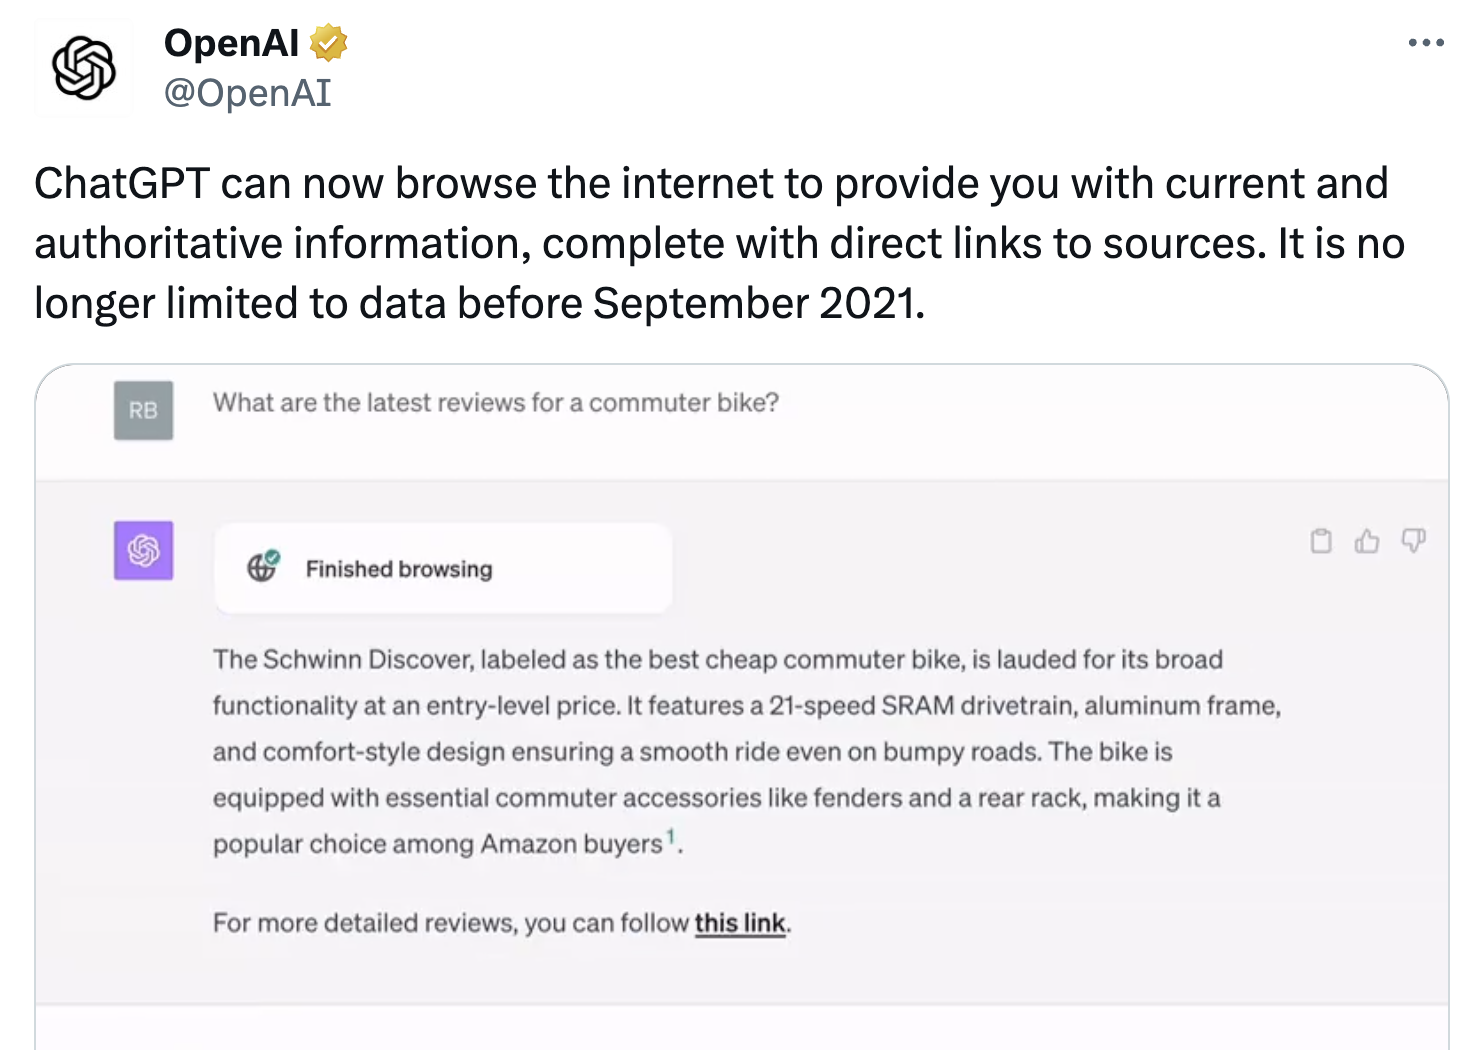
\includegraphics[height= 5.3in]{\images/retrieval}}

\slide{ChaptGPT as Therapist}

\centerline{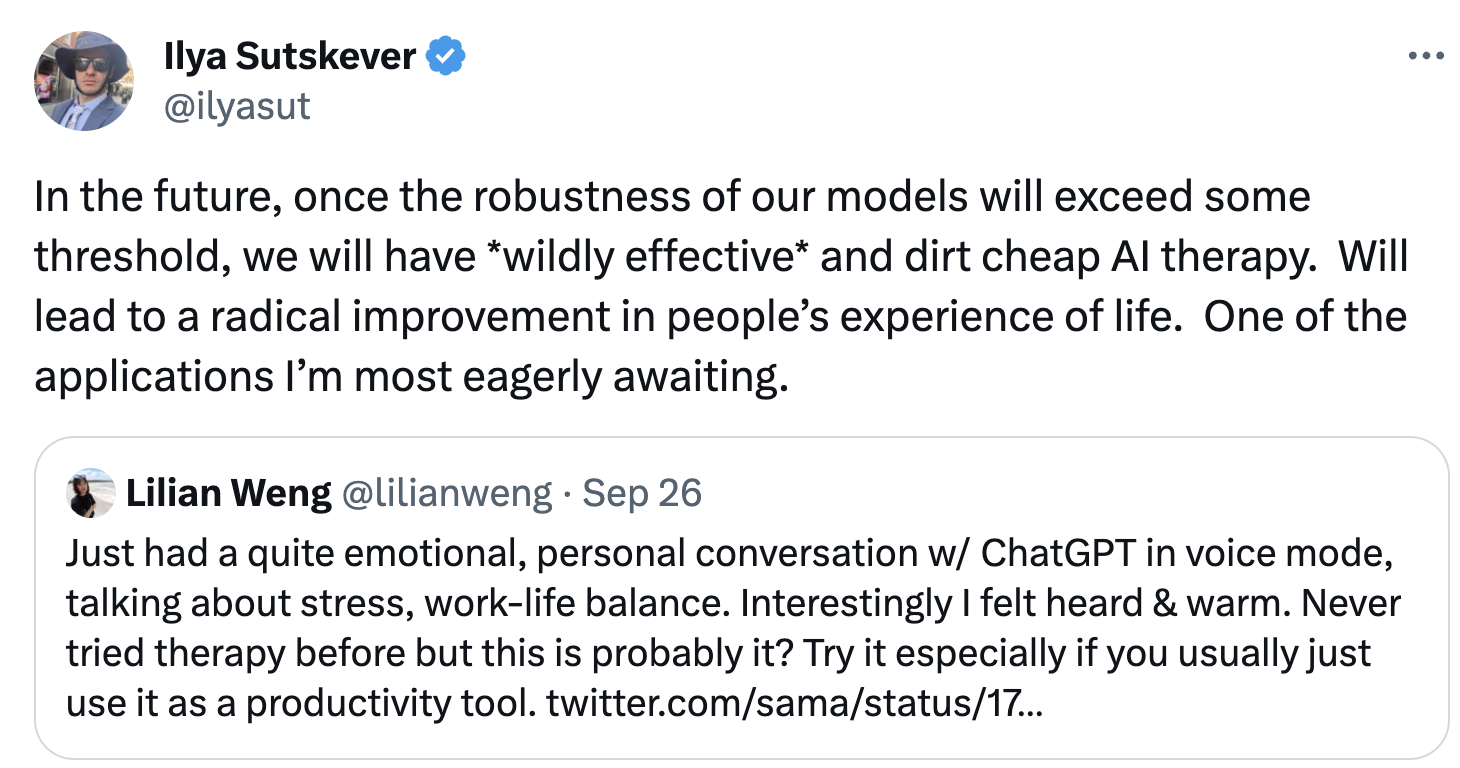
\includegraphics[height= 5in]{\images/Therapy}}


\slide{END}

}
\end{document}
